\documentclass[12pt,oneside,a4paper]{report}


\usepackage{lmodern}	       % Usa a fonte Latin Modern
\usepackage[table]{xcolor} 
\usepackage[utf8]{inputenc} % Suporte a UTF-8
\usepackage[T1]{fontenc}    % Fontes com suporte a caracteres especiais
\usepackage[portuguese]{babel} % Configuração para português
\usepackage{caption} % Para adicionar legendas
\usepackage[backend=biber, style=abnt]{biblatex} % Estilo ABNT
\usepackage{minted}
\usepackage{pdfpages}
\usepackage{multirow} % Adicione este pacote
\usepackage{chngcntr} % Para alterar a numeração dos contadores
\usepackage{changepage} % Para ajustar recuos
\usepackage{csquotes}       % Recomendado pelo biblatex para citações
\usepackage{setspace}       % Controle de espaçamento
\usepackage{ragged2e}       % Adiciona comandos para justificar texto
\usepackage{hyperref}       % Habilita links clicáveis
\usepackage{subcaption}   
\usepackage[font=small]{caption}
\usepackage{lastpage}			% Usado pela Ficha catalográfica
\usepackage{indentfirst}		% Indenta o primeiro parágrafo de cada seção.
\usepackage{color}				% Controle das cores
\usepackage{graphicx}			% Inclusão de gráficos
\usepackage{microtype} 			% para melhorias de justificação
\usepackage{xcolor} % Permite usar cores no texto
\usepackage{graphicx} % Para incluir imagens
\usepackage{float} % Para controle de posição das figuras

% Definir cores em tons pastel
\definecolor{color_200_200_200}{RGB}{200,200,200}
\definecolor{pastelBlue}{RGB}{135, 206, 250} % Azul pastel moderado
\definecolor{pastelOrange}{RGB}{255, 178, 102} % Laranja pastel equilibrado
\definecolor{pastelRed}{RGB}{240, 128, 128} % Vermelho pastel visível
\definecolor{pastelGreen}{RGB}{144, 238, 144} % Verde pastel

\usepackage{pifont}
\usepackage{amsmath}
\usepackage{amssymb,amsfonts,amsthm}
\usepackage{setspace}
\usepackage{pdfpages} 
\usepackage{hyperref}
\usepackage{adjustbox}
\usepackage{titling} % Para personalizar o título
\usepackage{titlesec}
\usepackage{tocloft} % Para controle do índice
\usepackage{geometry}
\usepackage{etoolbox}
\usepackage{xstring}
\usepackage{hyphenat}
\DeclareGraphicsExtensions{.png,.jpg,.pdf}

\titleformat{\chapter}[hang]
  {\normalfont\huge\bfseries}{}{0pt}{} % Define o estilo do título

% Ajustando as margens
\geometry{
  top=3cm,     % Margem superior de 2cm
  bottom=2cm,  % Margem inferior de 2cm
  left=3cm,    % Margem esquerda de 2cm
  right=2cm    % Margem direita de 2cm
}

% Configurações do Hyperref
\hypersetup{
    colorlinks=true,       % Links coloridos
    linkcolor=blue,        % Cor para links internos
    citecolor=blue2,        % Cor para citações
    urlcolor=blue,         % Cor para URLs
    filecolor=magenta,     
    breaklinks=true        % Permite que os links longos sejam quebrados
}
\definecolor{blue}{RGB}{41,5,195}
\definecolor{blue2}{RGB}{41,5,155}
% Ajuste para melhorar a quebra de links
\Urlmuskip=0mu plus 1mu

\addbibresource{bib.bib}    % Arquivo .bib com as referências 

% Justificar a bibliografia
\renewcommand*{\bibfont}{\sloppy\justifying\small\singlespacing}

% O tamanho do parágrafo é dado por:
\setlength{\parindent}{1.5cm}

% Controle do espaçamento entre um parágrafo e outro:
\setlength{\parskip}{1.5cm}  % tente também \onelineskip


% titulo central
\newcommand{\centersection}[1]{
    \begin{center}
        \textbf{\large #1}
    \end{center}
}
\counterwithout{figure}{chapter} % Remove a dependência de capítulos na numeração das figuras
\renewcommand{\listingscaption}{Código}
\renewcommand{\listoflistingscaption}{Lista de Códigos}


% Redefinindo o ambiente quote globalmente
\usepackage{etoolbox}
\AtBeginEnvironment{quote}{%
  \begin{adjustwidth}{4cm}{0cm} % Recuo de 4 cm à esquerda e nenhum ajuste à direita
  \fontsize{10}{12}\selectfont % Fonte com tamanho 10pt e espaçamento de linha 12pt
}

\AtEndEnvironment{quote}{
  \end{adjustwidth} % Fecha o ambiente adjustwidth
}
% Título do Trabalho
\newcommand{\titulo}{
 Tecnologias de Extração e Processamento de Informações Musicais em Musicoterapia: 
 Microanálises de Vestígios Musicais e possíveis interfaces com a Cognição Social }

% Nome do doutorando
\newcommand{\autor}{Ivan Moriá Borges Rodrigues}

% Nome da Instituição ao qual o polo Pertence
\newcommand{\instituicao}{Universidade Federal de Minas Gerais}

% Nome do Centro
\newcommand{\centro}{Escola de Música}

% Nome do Orientador
\newcommand{\orientador}{Renato Tocantins Sampaio}

% Nome do Co-orientador
\newcommand{\coorientador}{Sérgio Freire Garcia}

% Banca %
% Nome do Membro Interno
\newcommand{\membroInterno}{Frederico Gonçalves Pedrosa}
% Nome do Membro Externo
\newcommand{\membroExterno}{Claudia Regina de Oliveira Zanini}
\newcommand{\membroExternodois}{Luiz Rogério Jorgensen Carrer}
% Instituição do Membro Externo
\newcommand{\instituicaoExterno}{Universidade Federal de Goiás (UFG)}
\newcommand{\instituicaoExternodois}{Universidade Federal de São Paulo (UNIFESP)}

% Cidade onde ocorreu a defesa
\newcommand{\cidade}{Belo Horizonte}
% Estado onde Aconteceu a defesa
\newcommand{\estado}{MG}
% Mês da defesa
\newcommand{\mes}{Fevereiro}
% Dia da defesa
\newcommand{\dia}{7}
% Ano da defesa
\newcommand{\ano}{2025}

\graphicspath{{arquivos/figuras/}}

% Definindo os metadados do PDF
\hypersetup{
    pdftitle={Tecnologias de Extração e Processamento de Informações Musicais em Musicoterapia: Microanálises de Vestígios Musicais e possíveis interfaces com a Cognição Social},
    pdfauthor={Ivan Moriá Borges Rodrigues},
    pdfsubject={Tese de Doutorado em Música Univesidade Federal de Minas Gerais},
    pdfkeywords={Music Information Retrieval, Musicoterapia, Música e Tecnologia, Análise Musicoterapêutica}}

\begin{document}



\begin{center}
    \textsc{\instituicao}\\
    \textsc{\centro}\\
    \textsc{Programa de Pós-Graduação em Música}

    \vspace{4.5cm}
\autor\

    \begin{center}

    \vspace*{\fill} % Ajusta o espaço antes do título (aumenta ou diminui conforme necessário)
   \textbf{\titulo}
    \vspace*{\fill} % Ajusta o espaço depois do título
    \end{center}

    \vfill
    \cidade\ \\
    \ano\
\end{center}
\thispagestyle{empty} % Remove a numeração desta página
\newpage

\vspace{1cm}	

\begin{center}	
\textsc{\titulo}
\end{center}

\vspace{4.5cm}	

\begin{center}
\autor\
\end{center}

\begin{center}
    \vspace*{\fill} % Ajusta o espaço antes do título (aumenta ou diminui conforme necessário)
\hfill \parbox{8.5cm} 
{\noindent
Tese apresentada ao Programa de Pós-Graduação em Música, da \instituicao, como requisito parcial à obtenção do título de Doutor em Música.

\par{Linha de Pesquisa: Musicoterapia.}

\vspace{0.5cm}
Orientador: \orientador{}
\par Coorientador: \coorientador{}
}
\vfill

    \vspace*{\fill} % Ajusta o espaço depois do título
\end{center}

\begin{center}
\cidade\ \\
\ano\
\end{center}

\thispagestyle{empty} % Remove a numeração desta página
\newpage\


% Ficha Catalográfica
%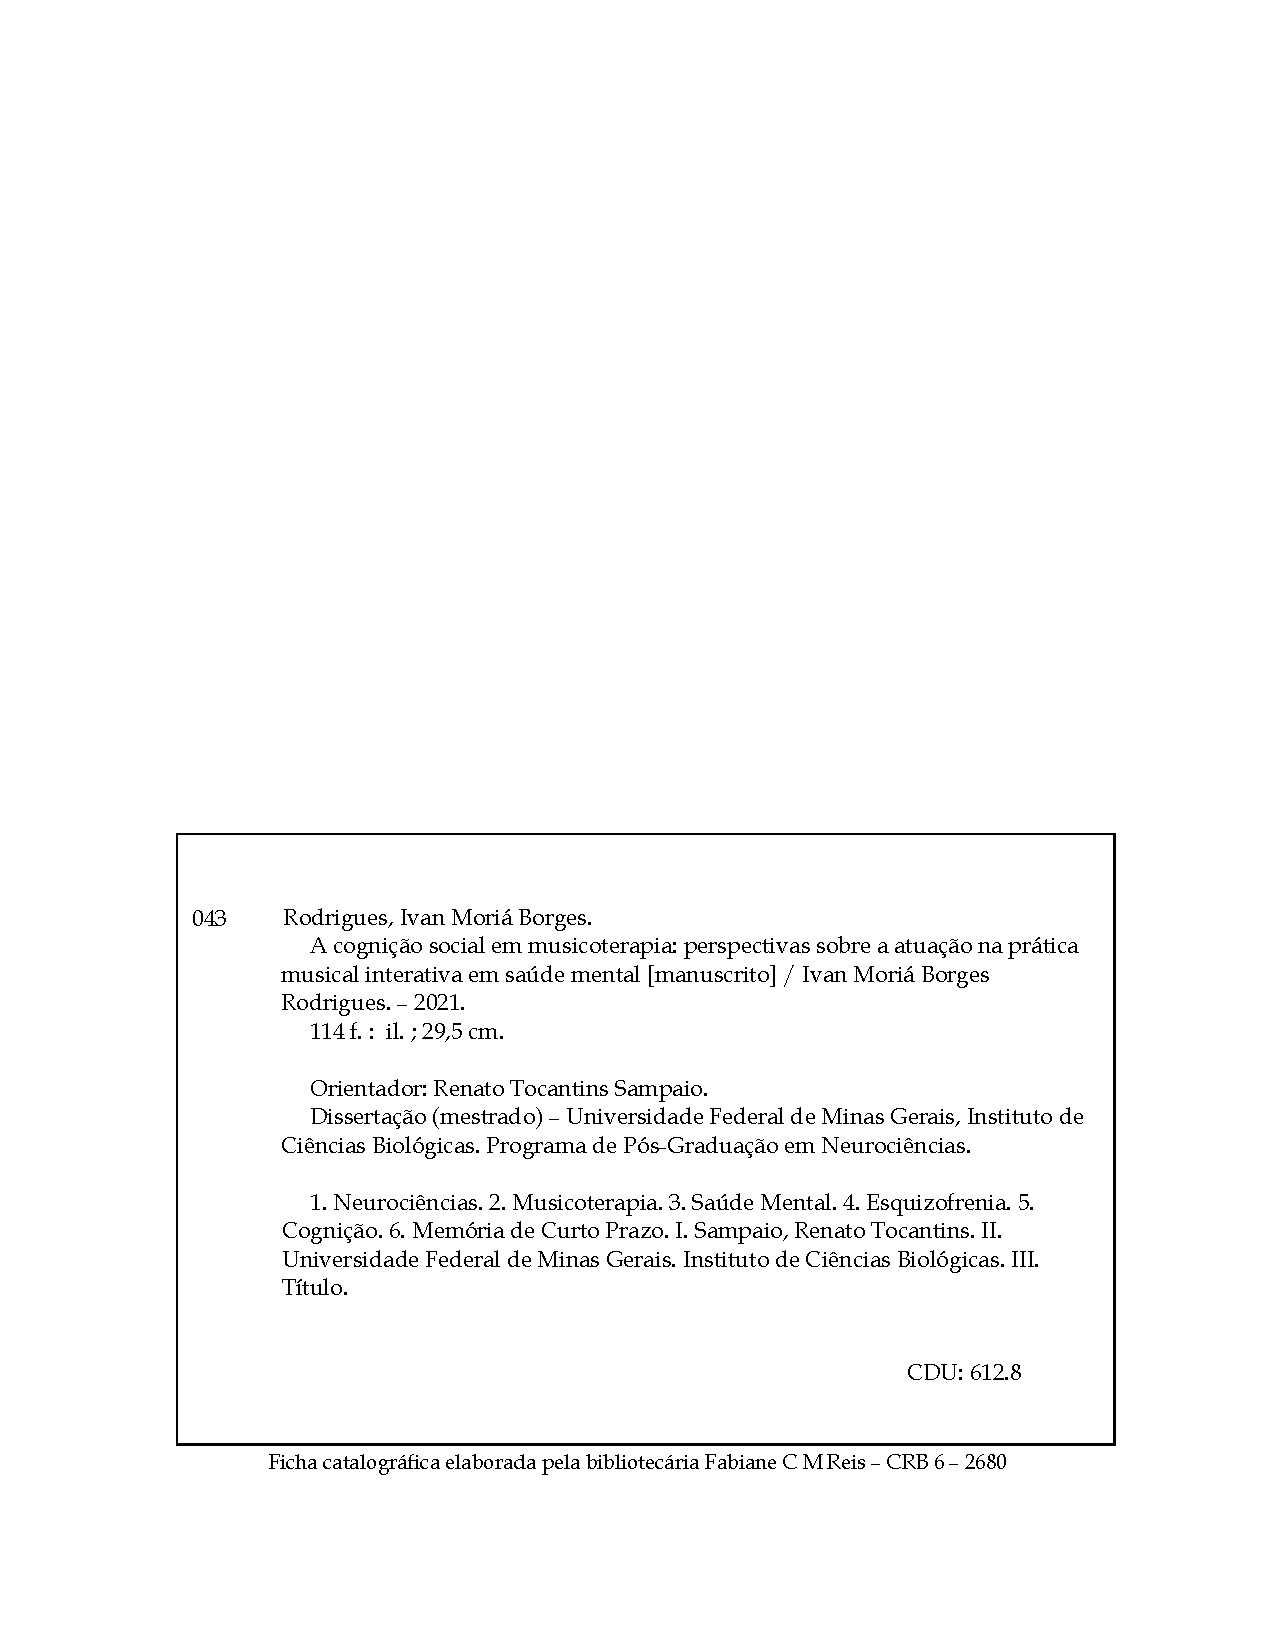
\includepdf{Arquivos/Ficha_Catalografica.pdf}

% -------------------------------------------------
% ELEMENTOS PRÉ-Textuais
% -------------------------------------------------

% Folha de aprovação 
%
\begin{figure}[h]
    \vspace{-2cm}
    \centering  
    
\includegraphics[scale=0.5]{Arquivos/Logo_Universidade.png}\label{fig:pesquisa}
\end{figure}


\begin{center}
    \vspace{0.5cm}
    \textsc{\instituicao}\\
    \textsc{\centro}\\
    \textsc{Programa de Pós-Graduação em Música}
\end{center}
\vspace{1cm}

 \noindent
Defesa da qualificação de doutorado de \textbf{\autor}, intitulada \textbf{\titulo} orientado pelo  \textbf{Prof\. Dr\. \orientador} e coorientado pelo  \textbf{Prof\. Dr\. \coorientador}, apresentado à banca examinadora designada pelo Colegiado do Programa de Pós-Graduação em Música da UFMG, em sete de fevereiro de 2025. Os membros da Banca Examinadora consideram o candidato:
 \rule{3cm}{0.5pt}  






\begin{center}
    \textbf{Banca Examinadora}\\
\vspace{0.8cm}
\rule{8cm}{0.5pt} 
\hfill

Prof\. Dr\. \orientador\ (orientador)\\
\instituicao\ (UFMG)

\vspace{1cm}
\rule{8cm}{0.5pt} \\
Prof\. Dr\. \coorientador\ (coorientador)\\
\instituicao\ (UFMG)
\vspace{1cm} \\
\rule{8cm}{0.5pt} \\
Profa\. Dra\. \membroExterno\  \\
\instituicaoExterno\ 
\vspace{1cm} \\
\rule{8cm}{0.5pt} \\
Prof\. Dr\. \membroExternodois\  \\
\instituicaoExternodois\ 
\vspace{1cm} \\
\rule{8cm}{0.5pt} \\
Prof\. Dr\. \membroInterno\ \\
\instituicao\ (UFMG)




\end{center} 





\vfill




\begin{center}

	\cidade\ \\
     \ano\
\end{center}

% \pagestyle{plain}
% \pagenumbering{roman}
\thispagestyle{empty} % Remove a numeração desta página

%\setcounter{page}{3} %Escolhe-se o estilo de numeração da página.
\newpage





% Dedicatória
\null\
\vfill

\hfill \parbox{4.0cm} {\noindent \textit{À Mônica Barbosa, por nunca desistir.}}
\thispagestyle{empty} % Remove a numeração desta página

\newpage


% Agradecimentos
\centersection{AGRADECIMENTOS} 





\pagenumbering{roman}  % Define a numeração romana
\setcounter{page}{1}  % Começa a numeração romana a partir de 1

\newpage


% Epígrafe
\null\
\vfill

\hfill \parbox{9.0cm} {\noindent Ora, a realidade é constituída por essências e existências particulares e, portanto, o conhecimento verdadeiro tem que ser um conhecimento que preserve o particular sem destruí-lo numa nomenclatura abstrata. 


\vspace{0.5cm}

\noindent Baruch de Espinosa}
\pagenumbering{roman}
\setcounter{page}{2}  % Começa a numeração romana a partir de 1



% Resumo

\centersection{RESUMO} 


\textbf{Palavras-chave}:
 

\pagenumbering{roman}
\setcounter{page}{3}  % Começa a numeração romana a partir de 1


\newpage



% Abstract

\centersection{ABSTRACT} % Cria o título
     
     Data collection for the analysis of music therapy sessions can be conducted in various ways. There is an abundance of qualitative studies that narrate the functioning of sessions observationally, supported by music therapy evaluation scales. There is a lack of publications in Brazil that utilize quantitative methods for data collection and analysis in Music Therapy using digital equipment, such as musical instruments that transmit information via MIDI (Musical Instrument Digital Interface) to electronic processing. This research project aims to identify the potential factors that hinder access to this form of data collection, explore ways to develop more accessible methods for use by music therapists in Brazil, and assess the feasibility of continuing to develop platforms that use MIDI technology for research. The methodology will be divided into two main workstreams. In the first, participants will interact through a digital MIDI instrument that processes all the musical information played, with musical elements in audio. All information will be processed in a patch developed in MAX/MSP for data collection and in a Python script for quantitative data analysis. In the second workstream, interviews will be conducted with music therapists who use technology in their practices, aiming to map the use of technological tools by music therapists and researchers and conduct an initial validity assessment of the material already developed. This will include initial studies of face, content, and construct validity of the developed protocol, such as analyses of correlations between spontaneous time and anxiety, correlations between synchronization error rates and anticipation skills (related to social cognition), among other psychometric analyses. We hope that this experiment will enable us to quantitatively visualize levels of perception among participants and the relationship between various musical stimuli and musical responses, specifically related to rhythmic aspects such as anticipation, delay, synchronization, perception, memory, and understanding of symbolic structures, among others. This project will contribute to the development of new tools for data collection in Music Therapy, also identifying potential factors that hinder access to this form of data collection and exploring ways to develop more accessible methods for use by music therapists in Brazil.
      
      
      
     \textbf{Keywords}: Music Information Retrieval, Music Therapy, Music and Technology, Music Therapy Analysis.




     \pagenumbering{roman}
     \setcounter{page}{4}  % Começa a numeração romana a partir de 1

  \newpage

% Lista de Figuras e Tabelas
%\addcontentsline{toc}{section}{Lista de Figuras} 
\listoffigures % Gera a lista de figuras
\newpage % Nova página para separar o conteúdo

%\addcontentsline{toc}{section}{Lista de Tabelas} 
\listoftables % Gera a lista de tabelas
\newpage % Nova página para separar o conteúdo

% Lista de Siglas
%Lista de Símbolos
% Lista de códigos
\listoflistings\newpage

% ------------------------------------
% SUMÁRIO
% ------------------------------------
\pdfbookmark[0]{\contentsname}{toc}
\tableofcontents
\cleardoublepage\pagenumbering{arabic}
\setcounter{page}{5}  % Começa a numeração romana a partir de 1

%-------------------------------------------------
% CAPÍTULOS
%-------------------------------------------------

%-------------------------------------------------
% Primeira Parte
\include{arquivos/capitulos/1}
%-------------------------------------------------

%Introdução
\include{arquivos/capitulos/motivos}

%Capítulo 1 - Prelude - Definindo conceitos
\include{arquivos/capitulos/intro}

% Restabelece a numeração de páginas a partir daqui
%\pagestyle{plain}
%Capítulo 2 - Allemande (MIR-MT)
\include{arquivos/capitulos/allemande}

%-------------------------------------------------
% Segunda Parte
\include{arquivos/capitulos/2}
%-------------------------------------------------
% Apresentar o software aqui como anexo

%Capítulo 2- Metodologia
\include{arquivos/capitulos/metodologia}

%-------------------------------------------------
% Terceira Parte
\include{arquivos/capitulos/3}
%-------------------------------------------------

% Capítulo 3 - Resultados
\include{arquivos/capitulos/resultados}

% Capítulo 3 - Discussão
\include{arquivos/capitulos/discussao}

% Capítulo 4 - Conclusão
\include{arquivos/capitulos/conclusao}

% REFERÊNCIAS BIBLIOGRÁFICAS 
\section{Bibliografia}
\printbibliography[heading=none]
\newpage

%  ITENS PÓS-TEXTUAIS  %
% Anexos
%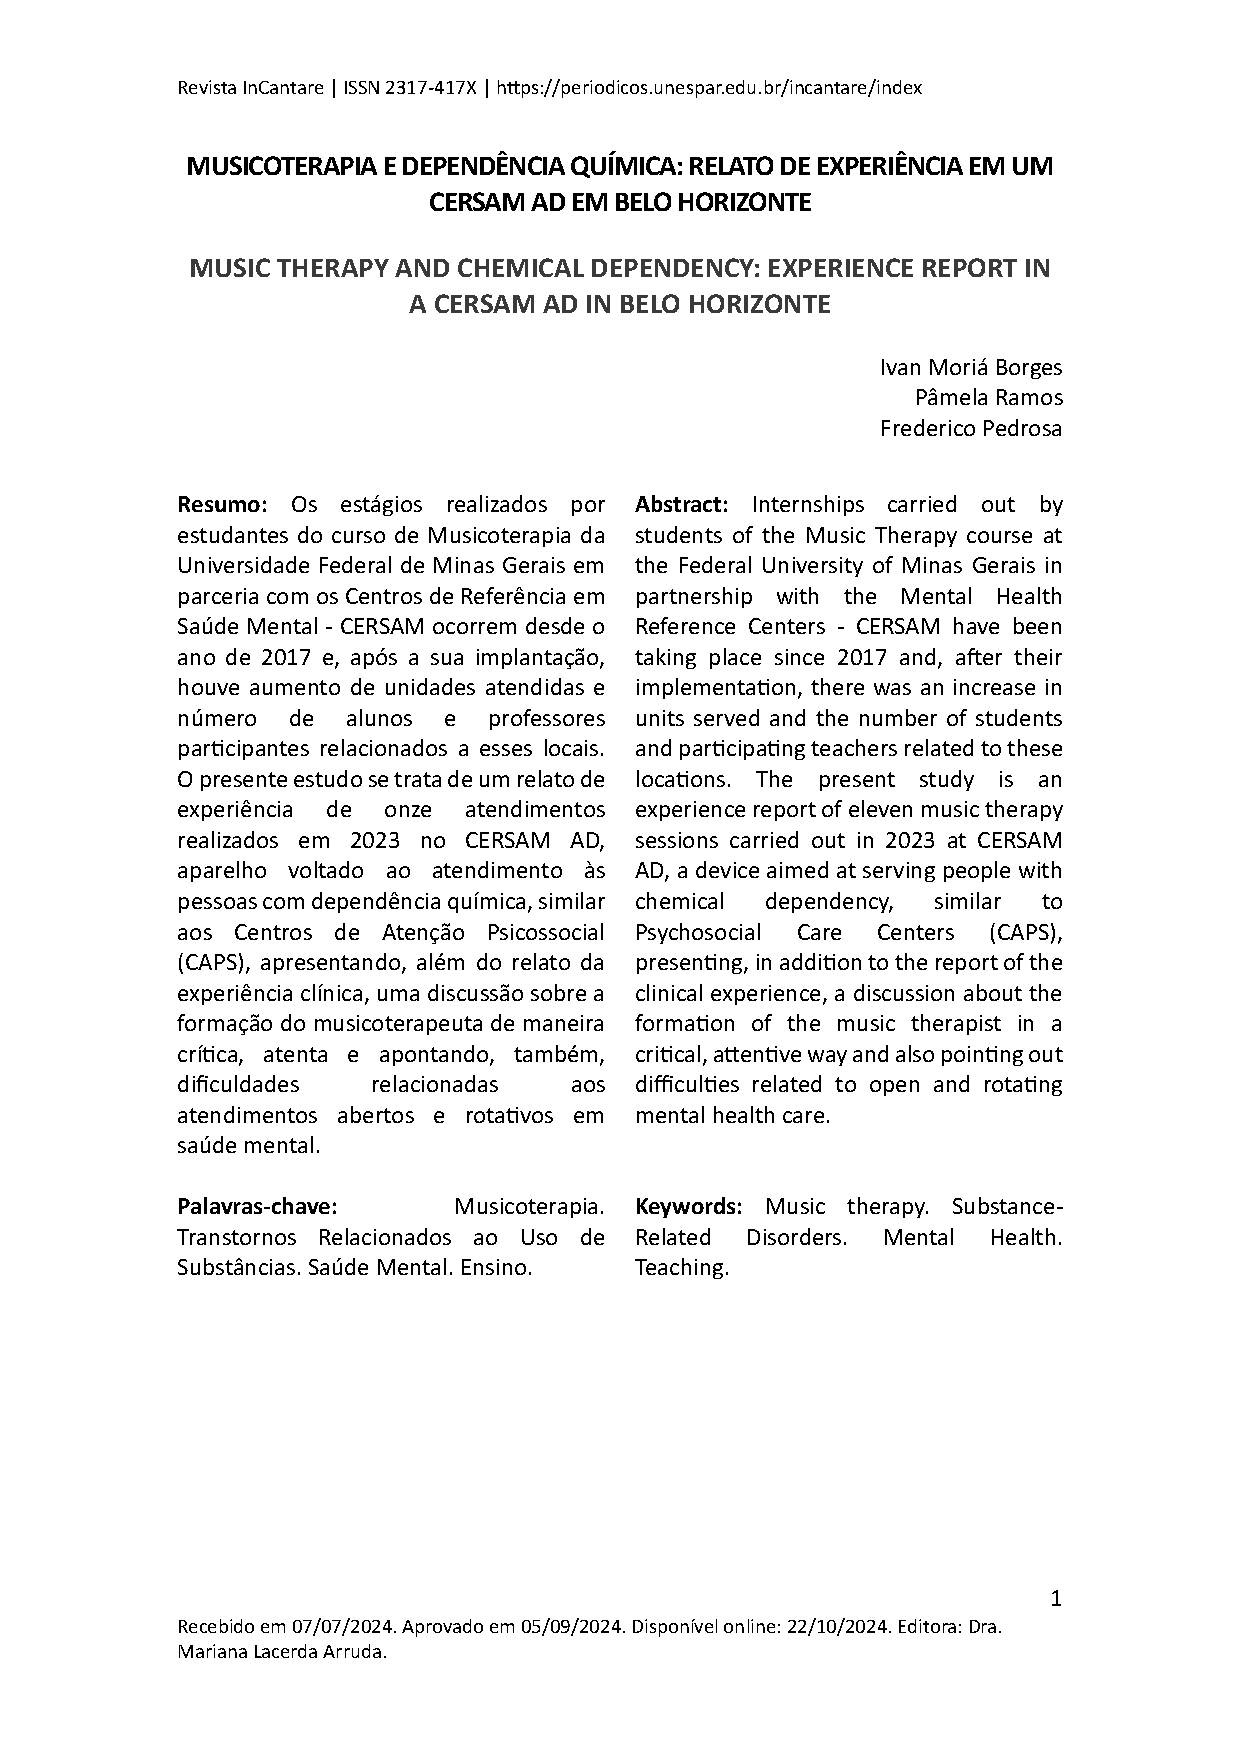
\includepdf[pages=-]{arquivos/anexos/artigoincantare.pdf}

% Apêndices

\end{document}
